\documentclass{article}

%%%%%%%%%%%%%%%%%%%%%%%%%%%%%%%%%%%%%%%%%%%%%%%%%%%%%%%%%%%%%%%%%%%%%%%

\usepackage{url}
\usepackage{graphicx}

%%%%%%%%%%%%%%%%%%%%%%%%%%%%%%%%%%%%%%%%%%%%%%%%%%%%%%%%%%%%%%%%%%%%%%%
%% Check these macro values for appropriateness for your own document.

\title{IS3 Group Report}

%%authors
\author{
  Richard Fleming \\
  James Gallagher \\
  Craig McLaughlin \\
  Victor Pantazi \\
  Ross Taylor \\
  Gordon Reid}

%%release date 
\date{\today}

%%%%%%%%%%%%%%%%%%%%%%%%%%%%%%%%%%%%%%%%%%%%%%%%%%%%%%%%%%%%%%%%%%%%%%%

\begin{document}

%%%%%%%%%%%%%%%%%%%%%%%%%%%%%%%%%%%%%%%%%%%%%%%%%%%%%%%%%%%%%%%%%%%%%%%

\maketitle

%%%%%%%%%%%%%%%%%%%%%%%%%%%%%%%%%%%%%%%%%%%%%%%%%%%%%%%%%%%%%%%%%%%%%%%
%% Standard section for all documents

\section{Preamble}

\subsection{In This Report}

\begin{itemize}
\item Give an overview of your paper prototypes, the early designs and
how you came to your final prototype design;

\item Explain how they work;

\item Report on your heuristic evaluation/think aloud, any problems you
found and how you resolved them (include the key paper prototypes that
you built);

\item Make a simple video of your final prototype (video from a phone
is fine) upload it to a video sharing site so we can see it in action.
I am not expecting Hollywood quality, but just enough to get an idea
of how your system would work. You can get some inspiration from the
video above;

\item Once your video is publicly available, send the link out to
friends and family and get them to comment in the public area and use
that information to create suggestions for improving the design.
\end{itemize}

\section{Overview}

Insert references in this text for the different calendars if they
have websites.

Our prototypes were based on the Facebook, OS X, Evolution on Scientific
Linux, and Google calendars. For prototyping and evaluating we split up
into two person teams. For the purposes of the discussion the teams are
labelled based on the calendars they evaluated.

The final paper prototype was a combination of our findings from the
calendars above and the design is illustrated in Figure~\ref{fig:fpp}.

\section{Calendar on OS X}

Paper prototype has minimalist design with three views: week, month,
and year. These views are available through three buttons that are
always on the screen at the top centre-right of the screen. The
currently selected view is colour/depressed differently than the
others.

Apple Inc.'s use of skeuomorphism creates an interface similar to a real 
calendar with simulated page rips, faux-leather textures for UI
elements, and page turn animations.

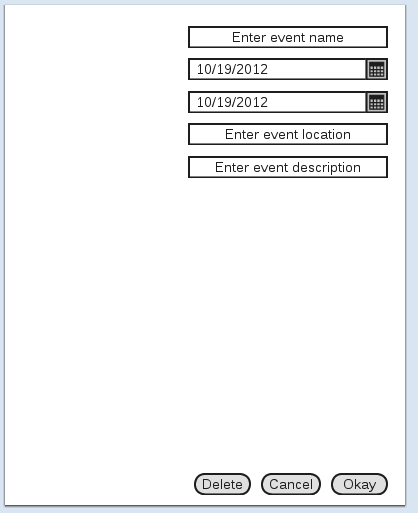
\includegraphics[scale=0.5]{CMCLGDREvent.png}

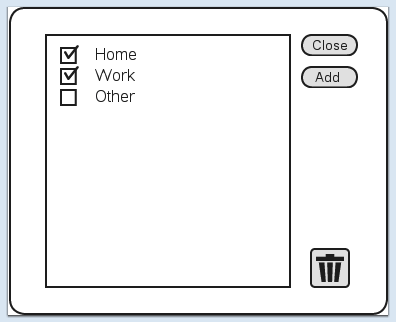
\includegraphics[scale=0.5]{CMCLGDRViewCalendar.png}

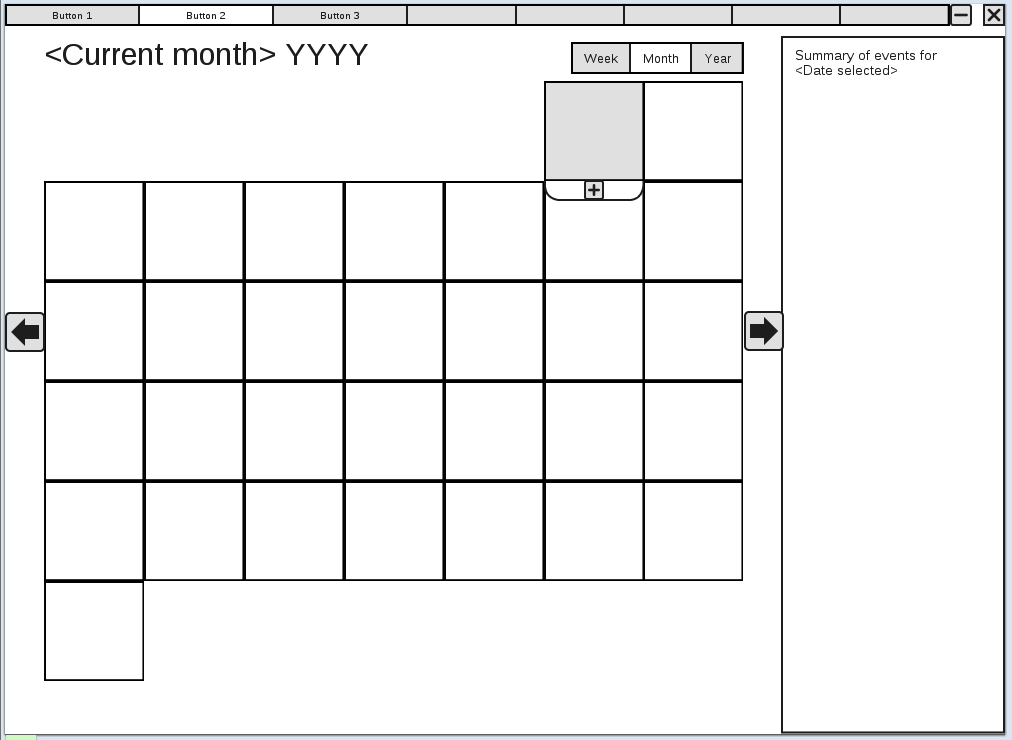
\includegraphics[scale=0.5,angle=90]{CMCLGDRMonth.png}

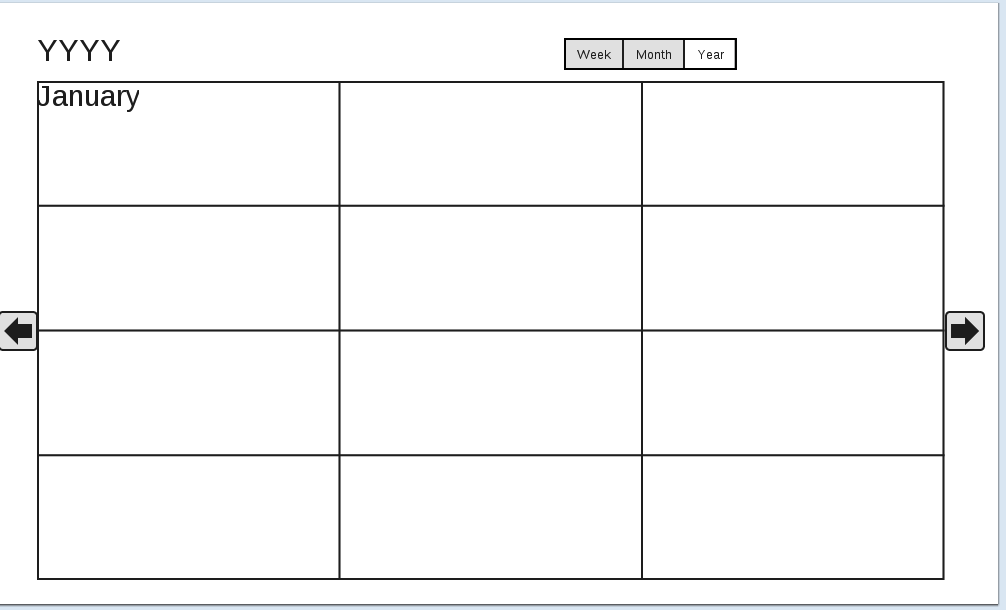
\includegraphics[scale=0.5,angle=90]{CMCLGDRYear.png}

\subsection{Problems during Evaluation}

The participant noted feeling uncomfortable during the evaluation as it
was unnatural for the them to have to vocalise their actions. At some
points during the experiment, the participant seemed confused or
surprised by the feedback from the system, occasionally expressing
uncertainty on how to proceed further with the task.

\section{Evolution on Scientific Linux}

This paper prototype was designed using our findings from our evaluation 
of Evolution on Scientific Linux.

The first thing we noticed about Evolution was that there wasn't always
a clear indication of the current system state so for our prototype we
included a clear `Day/Week/Month/Year' section at the top of the screen
which also allowed the user to quickly switch between views. Another
indicator of system state we added was a check box section on the left of
the main view to allow users to select different categories of event to
be displayed. Also related to event categories, we found Evolution's
system for adding a new category to be rather unintuitive so we added a
clear indication in the categories section of the sidebar labelled
'Add New'. We also didn't like the inconsistencies we found whilst
using the Evolution system so we decided the different views in our
prototype should have the same features available (i.e the sidebar
feature and the view indicator).

\subsection{Problems during Evaluation}

\begin{figure}
\centering
%\includegraphics[height=H,width=W]{finalpaperprototye.pdf}
\vspace{-50mm}
\caption{Final prototype design.}
\label{fig:ffp}
\end{figure}

%%%%%%%%%

See figures (need figures).
\section{The Video}

\url{http://www.youtube.com/watch?v=yAREKMqu538}

%% Separate sections with line of comment symbols.
%%%%%%%%%%%%%%%%%%%%%%%%%%%%%%%%%%%%%%%%%%%%%%%%%%%%%%%%%%%%%%%%%%%%%%%

\end{document}

%%%%%%%%%%%%%%%%%%%%%%%%%%%%%%%%%%%%%%%%%%%%%%%%%%%%%%%%%%%%%%%%%%%%%%%
